\documentclass[11pt]{article}

\usepackage[margin=1in]{geometry}
\usepackage[T1]{fontenc}
\usepackage{lmodern}
\usepackage{microtype}
\usepackage{amsmath,amssymb,amsthm,mathtools}
\usepackage{mathrsfs}
\usepackage[dvipsnames]{xcolor}
\usepackage[most]{tcolorbox}
\usepackage{graphicx}
\graphicspath{{figures/}{notes/figures/}}
\usepackage{tikz}
\usetikzlibrary{decorations.markings,patterns}
\usepackage{pgfplots}
\pgfplotsset{compat=1.17}
\usepackage{enumitem}
\usepackage{tocloft}
\usepackage[hidelinks]{hyperref}

\definecolor{courseblue}{HTML}{1F4E79}
\definecolor{lightblue}{HTML}{EAF2F8}
\definecolor{lightgreen}{HTML}{EAF7EA}
\definecolor{lightpink}{HTML}{FCE8EF}
\definecolor{lightyellow}{HTML}{FFF8D6}
\definecolor{warningyellow}{HTML}{D6A000}
\definecolor{exercisebg}{HTML}{FDEAEA}
\definecolor{exerciseframe}{HTML}{B54040}
\definecolor{examplebg}{HTML}{F4FAFE}
\definecolor{exampleframe}{HTML}{85C1E9}
\definecolor{darkgray}{HTML}{333333}
\definecolor{lightorange}{HTML}{FDEBD8}
\definecolor{orangeframe}{HTML}{E08A3C}
\definecolor{remarkbg}{HTML}{F3EEFB}
\definecolor{remarkframe}{HTML}{9B7FC9}
\definecolor{cayleyred}{HTML}{C0392B}
\definecolor{cayleygreen}{HTML}{1E8449}
\definecolor{cayleyblue}{HTML}{1F5FA0}
\definecolor{cayleyorange}{HTML}{D35400}
\definecolor{cayleypurple}{HTML}{7D3C98}
\definecolor{cayleyteal}{HTML}{117A65}

\setlength{\parindent}{0pt}
\setlength{\parskip}{0.45em}
\setlist[itemize]{topsep=0.25em,itemsep=0.15em}
\renewcommand{\cftsecleader}{\cftdotfill{\cftdotsep}}
\renewcommand{\cftsubsecleader}{\cftdotfill{\cftdotsep}}

\theoremstyle{plain}
\newtheorem{theorem}{Theorem}[section]
\newtheorem{proposition}[theorem]{Proposition}
\newtheorem{lemma}[theorem]{Lemma}
\newtheorem{corollary}[theorem]{Corollary}
\theoremstyle{definition}
\newtheorem{definition}[theorem]{Definition}
\newtheorem{example}[theorem]{Example}
\newtheorem{exercise}[theorem]{Exercise}
\newtheoremstyle{boldremark}
  {3pt}{3pt}{\normalfont}{}{\bfseries}{.}{.5em}
  {\thmname{#1}\thmnumber{ #2}\thmnote{ (#3)}}
\theoremstyle{boldremark}
\newtheorem*{remark}{Remark}
\theoremstyle{remark}
\newtheorem*{fact}{Fact}
\newtheorem*{warning}{Warning}

\tcolorboxenvironment{definition}{
  enhanced,
  unbreakable,
  colback=lightgreen,
  colframe=ForestGreen,
  boxrule=0.7pt,
  arc=2pt,
  left=6pt,
  right=6pt,
  top=5pt,
  bottom=5pt
}

\tcolorboxenvironment{remark}{
  enhanced,
  colback=remarkbg,
  colframe=remarkframe,
  before upper={\setlength{\parskip}{0.5em}},
  boxrule=0.7pt,
  arc=2pt,
  left=6pt,
  right=6pt,
  top=5pt,
  bottom=5pt
}

\tcolorboxenvironment{warning}{
  enhanced,
  colback=lightyellow,
  colframe=warningyellow,
  boxrule=0.7pt,
  arc=2pt,
  left=6pt,
  right=6pt,
  top=5pt,
  bottom=5pt
}

\tcolorboxenvironment{exercise}{
  enhanced,
  colback=exercisebg,
  colframe=exerciseframe,
  boxrule=1pt,
  arc=2pt,
  left=6pt,
  right=6pt,
  top=5pt,
  bottom=5pt
}

\tcolorboxenvironment{example}{
  enhanced,
  colback=examplebg,
  colframe=exampleframe,
  boxrule=0.7pt,
  arc=2pt,
  left=6pt,
  right=6pt,
  top=5pt,
  bottom=5pt
}

\numberwithin{equation}{section}

\newcommand{\be}{\begin{eqnarray}}
\newcommand{\ee}{\end{eqnarray}}
\newcommand{\C}{\mathbb{C}}
\newcommand{\R}{\mathbb{R}}
\newcommand{\N}{\mathbb{N}}
\newcommand{\Z}{\mathbb{Z}}
\DeclareMathOperator{\Log}{Log}
\DeclareMathOperator{\Arg}{Arg}

\DeclareMathOperator{\Hol}{\mathcal{H}\mathrm{ol}}
\DeclareMathOperator{\Real}{Re}
\DeclareMathOperator{\Imag}{Im}
\newcommand{\A}{\mathcal{A}}
\newcommand{\CT}{\C[[T]]}
\newcommand{\CLT}{\C((T))}
\tcbset{breakable}
% Compact spacing around diagrams; keep the main text at 11pt.
\newenvironment{lecturefigure}
 {\par\addvspace{0.25em}\begingroup\setlength{\parskip}{0pt}\centering}
 {\par\endgroup\addvspace{0.25em}}
\begin{document}

\begin{center}
  \colorbox{lightblue}{%
    \begin{minipage}{0.94\textwidth}
      \vspace{0.55em}
      \begin{tabular*}{\textwidth}{@{\extracolsep{\fill}}lr}
        {\color{courseblue}\bfseries\LARGE Lecture 32} &
        {\color{courseblue}\bfseries\LARGE MATH 411}\\[0.35em]
        \textbf{Fall 2026} & \textbf{Date: Dec 2, 2026}\\
        & \textbf{Instructor: Manish Patnaik}
      \end{tabular*}
      \vspace{0.45em}
    \end{minipage}}
\end{center}

\setcounter{tocdepth}{1}
\tableofcontents
\vspace{0.45em}

% Source: handwritten Lecture 31, Dec. 2, pp. 1--7.
\section{Analytic continuation}

In Lecture~31 we introduced two functions initially defined only on right
half-planes: the Riemann zeta function $\zeta(s)=\sum_{n=1}^{\infty} n^{-s}$
on $\{\Real s > 1\}$, and the Gamma function
$\Gamma(s)=\int_0^{\infty} e^{-t}t^{s-1}\,dt$ on $\{\Real s > 0\}$. We now
make precise what it means to extend such a function to all of $\C$.

\begin{definition}[Analytic continuation as a meromorphic function]
Let $a\in\R$, and let $f(z)$ be a holomorphic function on the right
half-plane $H_a=\{z\in\C:\Real z > a\}$. We say that $f$ has an
\emph{analytic continuation to $\C$ as a meromorphic function} if there
exists a meromorphic function $g$ on $\C$ such that
\[
 g(z) = f(z) \qquad \text{for all } z\in\C \text{ with } \Real z > a.
\]
\end{definition}

\begin{lecturefigure}
\begin{minipage}{\linewidth}\centering
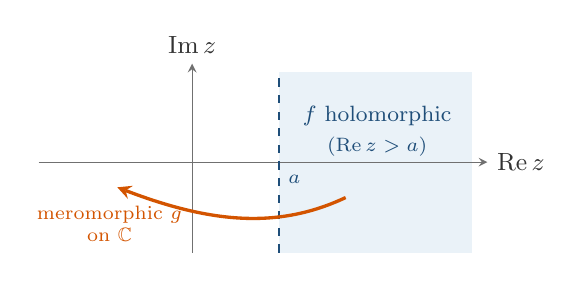
\begin{tikzpicture}[>=stealth,font=\small]
 \fill[lightblue] (1.1,-1.15) rectangle (3.55,1.15);
 \draw[darkgray!70,->] (-1.95,0) -- (3.75,0) node[right,text=darkgray] {$\Real z$};
 \draw[darkgray!70,->] (0,-1.15) -- (0,1.25) node[above,text=darkgray] {$\Imag z$};
 \draw[courseblue,dashed,thick] (1.1,-1.15) -- (1.1,1.15);
 \node[below right,font=\scriptsize,text=courseblue] at (1.1,-0.04) {$a$};
 \node[text=courseblue,font=\footnotesize] at (2.35,0.58) {$f$ holomorphic};
 \node[text=courseblue,font=\scriptsize] at (2.35,0.20) {$(\Real z > a)$};
 \draw[->,cayleyorange,very thick]
  (1.95,-0.45) .. controls (1.1,-0.85) and (0.25,-0.78) .. (-0.95,-0.32);
 \node[text=cayleyorange,font=\scriptsize,align=center] at (-1.05,-0.78) {meromorphic $g$\\on $\C$};
\end{tikzpicture}

\vspace{0.15em}
{\small Extending a holomorphic function $f$ from a right half-plane
$\{\Real z > a\}$ to a meromorphic function $g$ on $\C$.}
\end{minipage}
\end{lecturefigure}

\begin{remark}[Key properties of analytic continuation]
\leavevmode
\begin{enumerate}[label=\textup{(\arabic*)}]
 \item \textbf{Poles are allowed:} An analytic continuation as above need
       not be holomorphic everywhere on $\C$; it is only required to be
       meromorphic, so it may have isolated poles in $\{\Real z \leq a\}$.
 \item \textbf{Uniqueness:} If $g_1$ and $g_2$ are two meromorphic
       continuations of $f$ to $\C$, then $g_1=g_2$ everywhere on $\C$.
       Indeed, $g_1-g_2$ is meromorphic on $\C$ and vanishes identically on
       the open half-plane $\{\Real z > a\}$, so by the isolated-zero
       principle (Lecture~10 and Lecture~25), $g_1-g_2\equiv 0$ on $\C$.
\end{enumerate}
\end{remark}

\begin{example}[The zeta and Gamma functions]
\leavevmode
\begin{itemize}
 \item The Riemann zeta function $\zeta(s)=\sum_{n=1}^{\infty} n^{-s}$
       ($\Real s > 1$) admits a meromorphic continuation to all of $\C$
       whose only pole is a simple pole at $s=1$.
 \item The Gamma function $\Gamma(s)=\int_0^{\infty} e^{-t}t^s\,\frac{dt}{t}$
       ($\Real s > 0$) admits a meromorphic continuation to all of $\C$
       with simple poles at $s=0,-1,-2,\dots$.
\end{itemize}
\end{example}

\begin{warning}
Knowing that $\zeta(s)$ continues meromorphically to $\C\setminus\{1\}$
does \emph{not} mean that $\zeta(s)=\sum_{n=1}^{\infty} n^{-s}$ holds for
all $s\in\C\setminus\{1\}$. The Dirichlet series diverges whenever
$\Real s\leq 1$; analytic continuation produces a different expression on
$\C$ that coincides with the series on $\{\Real s > 1\}$.
\end{warning}

Our plan for this lecture and the next is twofold:
\begin{enumerate}[label=\textup{(\arabic*)}]
 \item explain why $\zeta(s)$ and its analytic continuation are central to
       the distribution of prime numbers;
 \item carry out the analytic continuation of $\Gamma(s)$ today, and use it
       together with theta inversion in Lecture~33 to continue $\zeta(s)$.
\end{enumerate}


\section{The Euler product, primes, and the Prime Number Theorem}

Why does $\zeta(s)$ tell us anything about prime numbers? The link is an
identity discovered by Euler that expresses $\zeta(s)$ as an infinite
product indexed by all prime numbers.

\begin{theorem}[Euler product formula]\label{thm:euler-product}
For every $s\in\C$ with $\Real s > 1$,
\begin{equation}\label{eq:euler-product}
 \boxed{\displaystyle
  \zeta(s) = \prod_{p\text{ prime}} \frac{1}{1-p^{-s}}.}
\end{equation}
\end{theorem}

\begin{proof}
Fix $s\in\C$ with $\sigma=\Real s > 1$. For every prime $p$, we have
$|p^{-s}|=p^{-\sigma}<1$, so the geometric series formula
$(1-x)^{-1}=\sum_{k=0}^{\infty} x^k$ ($|x|<1$) gives
\[
 \frac{1}{1-p^{-s}}
 = 1 + p^{-s} + (p^2)^{-s} + (p^3)^{-s} + \cdots
 = \sum_{k=0}^{\infty} (p^k)^{-s},
\]
with absolute convergence.

Let $p_1 < p_2 < p_3 < \cdots$ list all primes in increasing order. For any
integer $N\geq 1$, multiply the absolutely convergent geometric series for
the first $N$ primes:
\begin{align*}
 \prod_{j=1}^{N}\frac{1}{1-p_j^{-s}}
 &= \bigl(1 + p_1^{-s} + p_1^{-2s} + \cdots\bigr)
    \bigl(1 + p_2^{-s} + p_2^{-2s} + \cdots\bigr)
    \cdots
    \bigl(1 + p_N^{-s} + p_N^{-2s} + \cdots\bigr) \\
 &= \sum_{a_1,\dots,a_N \geq 0}
    \bigl(p_1^{a_1} p_2^{a_2}\cdots p_N^{a_N}\bigr)^{-s}.
\end{align*}
By the Fundamental Theorem of Arithmetic, every positive integer $n$ factors
uniquely as a product of prime powers. Hence as $(a_1,\dots,a_N)$ runs over
all $N$-tuples of nonnegative integers, the products
$p_1^{a_1}\cdots p_N^{a_N}$ hit each positive integer in the set
\[
 S_N = \{n\in\N : \text{every prime factor of } n \text{ belongs to }
        \{p_1,\dots,p_N\}\}
\]
\emph{exactly once}. Therefore,
\[
 \prod_{j=1}^{N}\frac{1}{1-p_j^{-s}} = \sum_{n\in S_N}\frac{1}{n^s}.
\]
Notice that every integer $n$ with $1\leq n\leq p_N$ has all its prime
factors $\leq p_N$, so $\{1,2,\dots,p_N\}\subseteq S_N$. Consequently,
\[
 \left|\zeta(s) - \prod_{j=1}^{N}\frac{1}{1-p_j^{-s}}\right|
 = \left|\sum_{n\notin S_N}\frac{1}{n^s}\right|
 \leq \sum_{n > p_N}\frac{1}{n^{\sigma}} \xrightarrow[N\to\infty]{} 0,
\]
because $\sum_{n=1}^{\infty} n^{-\sigma} < \infty$ for $\sigma > 1$ and
$p_N\to\infty$ (there are infinitely many primes). Taking $N\to\infty$
gives \eqref{eq:euler-product}.
\end{proof}

\begin{remark}[Euler's proof that there are infinitely many primes]
In fact, the finite-product identity above already implies that there are
infinitely many primes: if $\{p_1,\dots,p_N\}$ were the set of \emph{all}
primes, then $S_N=\N$ and for every real $s>1$ we would have
$\sum_{n=1}^{\infty} n^{-s} = \prod_{j=1}^{N}(1-p_j^{-s})^{-1}$. Letting
$s\to 1^+$, the right-hand side approaches the finite number
$\prod_{j=1}^{N}(1-p_j^{-1})^{-1}$, whereas the left-hand side diverges to
$+\infty$ (since the harmonic series diverges), a contradiction.
\end{remark}

We can ask much more than whether there are infinitely many primes: how
densely are they distributed?

\begin{definition}[Prime counting function]
For any positive real number $x>0$, let
\[
 \pi(x) = \#\{\text{primes } p \leq x\}
\]
denote the number of primes not exceeding $x$.
\end{definition}

The asymptotic growth of $\pi(x)$ is described by one of the landmark
theorems of nineteenth-century mathematics, proved independently in 1896 by
Hadamard and de la Vall\'ee Poussin using complex analysis.

\begin{theorem}[Prime Number Theorem, 1896]
As $x\to\infty$,
\[
 \boxed{\displaystyle
  \pi(x) \sim \frac{x}{\log x},
  \qquad\text{meaning}\qquad
  \lim_{x\to\infty}\frac{\pi(x)}{x/\log x} = 1.}
\]
\end{theorem}

How does analytic continuation of $\zeta(s)$ enter the picture? Assume that
$\zeta(s)$ has been meromorphically continued to $\C$ with its only pole at
$s=1$. Then $\zeta(s)$ is defined and holomorphic everywhere along the
vertical line $\Real s = 1$ except at $s=1$ itself.

\begin{fact}
The meromorphic continuation of $\zeta(s)$ has \emph{no zeros} on the line
$\Real s = 1$.
\end{fact}

In fact, the Prime Number Theorem is closely tied to this nonvanishing
property:
\[
 \text{Prime Number Theorem}
 \quad\Longleftrightarrow\quad
 \zeta(s) \text{ does not vanish on } \Real s = 1.
\]
We will prove in Lecture~33 that $\zeta(1+it)\neq 0$ for all $t\neq 0$, and
outline how this leads to the Prime Number Theorem.

Going a step further, write
\[
 \pi(x) = \frac{x}{\log x} + E(x),
\]
where $E(x)$ is the error term (more precisely, one compares $\pi(x)$ with
$\operatorname{Li}(x)=\int_2^x \frac{dt}{\log t}\sim \frac{x}{\log x}$).
Asking whether the error term is as small as probabilistic heuristics
predict is equivalent to the most famous open problem in mathematics:

\begin{remark}[The Riemann Hypothesis]
The \emph{Riemann Hypothesis} asserts that the only zeros of $\zeta(s)$
inside the \emph{critical strip} $0\leq\Real s\leq 1$ lie on the
\emph{critical line} $\Real s = \tfrac12$. Roughly speaking, the farther
to the left of $\Real s = 1$ we know $\zeta(s)$ is zero-free, the sharper
the error bound on $\pi(x)$; the Riemann Hypothesis corresponds to the
optimal square-root error bound.
\end{remark}

\begin{lecturefigure}
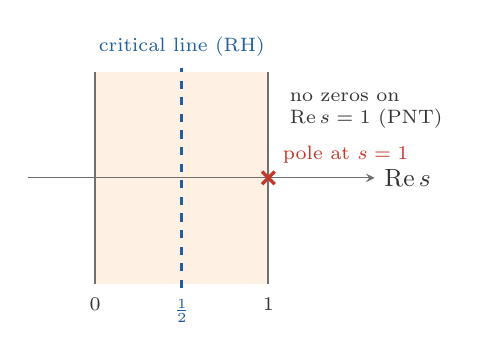
\begin{tikzpicture}[>=stealth,font=\small]
 \fill[lightorange!70] (0,-1.35) rectangle (2.2,1.35);
 \draw[darkgray!70,->] (-0.85,0) -- (3.55,0) node[right,text=darkgray] {$\Real s$};
 \draw[darkgray!70,thick] (0,-1.35) -- (0,1.35);
 \draw[cayleyblue,dashed,very thick] (1.1,-1.40) -- (1.1,1.40);
 \draw[darkgray!70,thick] (2.2,-1.35) -- (2.2,1.35);
 % Pole at s=1 marked with red x
 \draw[cayleyred,very thick] (2.2-0.08,-0.08) -- (2.2+0.08,0.08);
 \draw[cayleyred,very thick] (2.2-0.08,0.08) -- (2.2+0.08,-0.08);
 % Labels
 \node[below,font=\scriptsize,text=darkgray] at (0,-1.40) {$0$};
 \node[below,font=\scriptsize,text=cayleyblue] at (1.1,-1.42) {$\tfrac12$};
 \node[below,font=\scriptsize,text=darkgray] at (2.2,-1.40) {$1$};
 \node[above right,font=\scriptsize,text=cayleyred] at (2.26,0.06) {pole at $s=1$};
 \node[right,font=\scriptsize,text=darkgray,align=left] at (2.35,0.85)
  {no zeros on\\$\Real s = 1$ (PNT)};
 \node[above,font=\scriptsize,text=cayleyblue] at (1.1,1.42) {critical line (RH)};
\end{tikzpicture}

{\small The critical strip $0\leq\Real s\leq 1$: nonvanishing on
$\Real s=1$ drives the Prime Number Theorem; the Riemann Hypothesis places
all zeros in the strip on $\Real s=\tfrac12$.}
\end{lecturefigure}


\section{Morera's theorem and parameter-dependent integrals}

Before continuing $\Gamma(s)$ and $\zeta(s)$, let us revisit the
holomorphicity of parameter-dependent integrals from Lecture~31 using
\emph{Morera's theorem} (Lecture~21), which gives a very direct and
transparent proof.

\begin{proposition}[Holomorphicity on a finite interval]\label{prop:finite-int-hol}
Let $I=[a,b]\subset\R$ be a finite closed interval, let $U\subseteq\C$ be
open, and let $f:I\times U\to\C$ be continuous in $(t,z)$. Suppose that for
each fixed $t\in I$, the function $z\mapsto f(t,z)$ is holomorphic on $U$.
Then
\[
 F(z) = \int_I f(t,z)\,dt
\]
is holomorphic on $U$.
\end{proposition}

\begin{proof}
Fix any open disc $D$ with $\overline{D}\subset U$. Since $I\times\overline{D}$
is compact, $f$ is uniformly continuous there, which implies that $F$ is
continuous on $D$.

Recall Morera's theorem (Lecture~21): a continuous function $F$ on a disc
$D$ is holomorphic on $D$ if $\int_{\partial R} F(z)\,dz = 0$ for every
closed rectangle $R\subset D$.

\begin{lecturefigure}
\begin{minipage}{\linewidth}\centering
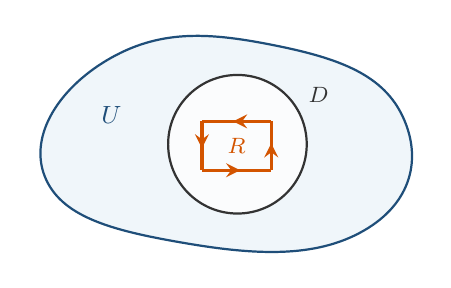
\begin{tikzpicture}[>=stealth,font=\small,
 midarrow/.style={postaction={decorate},decoration={markings,mark=at position .55 with {\arrow{>}}}}]
 % Domain U
 \fill[lightblue!70] plot[smooth cycle,tension=0.8] coordinates
  {(-2.2,-0.35) (-1.35,1.15) (0.75,1.3) (2.35,0.4) (1.85,-1.05) (-0.45,-1.2)};
 \draw[courseblue,thick] plot[smooth cycle,tension=0.8] coordinates
  {(-2.2,-0.35) (-1.35,1.15) (0.75,1.3) (2.35,0.4) (1.85,-1.05) (-0.45,-1.2)};
 \node[courseblue] at (-1.35,0.42) {$U$};
 % Disc D
 \fill[white,fill opacity=0.75] (0.25,0.05) circle (0.88);
 \draw[darkgray,thick] (0.25,0.05) circle (0.88);
 \node[darkgray,font=\footnotesize] at (1.28,0.68) {$D$};
 % Rectangle R inside D
 \draw[cayleyorange,very thick,midarrow] (-0.20,-0.28) -- (0.68,-0.28);
 \draw[cayleyorange,very thick,midarrow] (0.68,-0.28) -- (0.68,0.34);
 \draw[cayleyorange,very thick,midarrow] (0.68,0.34) -- (-0.20,0.34);
 \draw[cayleyorange,very thick,midarrow] (-0.20,0.34) -- (-0.20,-0.28);
 \node[cayleyorange,font=\footnotesize] at (0.24,0.03) {$R$};
\end{tikzpicture}

\vspace{0.15em}
{\small Testing holomorphicity of $F(z)=\int_I f(t,z)\,dt$ on $D\subset U$
via Morera's theorem on rectangles $R\subset D$.}
\end{minipage}
\end{lecturefigure}

Let $R\subset D$ be any closed rectangle. Since $(t,z)\mapsto f(t,z)$ is
continuous on the compact set $I\times\partial R$, we may interchange the
order of integration:
\[
 \int_{\partial R} F(z)\,dz
 = \int_{\partial R}\left(\int_I f(t,z)\,dt\right)dz
 = \int_I \left(\int_{\partial R} f(t,z)\,dz\right)dt.
\]
For each fixed $t\in I$, the function $z\mapsto f(t,z)$ is holomorphic on
$D$, so Cauchy's theorem gives $\int_{\partial R} f(t,z)\,dz = 0$.
Therefore $\int_{\partial R} F(z)\,dz = 0$ for every rectangle $R\subset D$.
By Morera's theorem, $F$ is holomorphic on $D$; since $D\subset U$ was
arbitrary, $F$ is holomorphic on $U$.
\end{proof}

\textbf{Applying this to $\Gamma(s)$.}
For $\Gamma(s)=\int_0^{\infty} e^{-t}t^{s}\,\frac{dt}{t}$ on
$U=\{s\in\C:\Real s > 0\}$, the interval $I=(0,\infty)$ is infinite (and
open at $0$, where $t^{s-1}$ blows up when $0<\Real s < 1$). To bridge from
Proposition~\ref{prop:finite-int-hol} to $(0,\infty)$, approximate $\Gamma$
using the compact subintervals $I_n=[1/n, n]$ ($n\geq 1$):
\[
 F_n(s) = \int_{1/n}^{n} e^{-t}t^{s}\,\frac{dt}{t}.
\]
By Proposition~\ref{prop:finite-int-hol}, each $F_n$ is holomorphic on $U$.
In Lecture~31 (Proposition~4.2), we proved that $F_n\to\Gamma$ uniformly on
every compact subset of $U$. In particular, for any closed rectangle $R$ in
a disc $D\subset U$, uniform convergence on $\partial R$ gives
\[
 \int_{\partial R}\Gamma(s)\,ds
 = \lim_{n\to\infty}\int_{\partial R} F_n(s)\,ds = 0,
\]
and Morera's theorem again confirms that $\Gamma(s)$ is holomorphic for
$\Real s > 0$.


\section{Analytic continuation of the Gamma function}

Recall from Lecture~31 (Proposition~4.3) that for $\Real s > 0$, $\Gamma(s)$
satisfies the functional equation
\begin{equation}\label{eq:gamma-shift}
 s\,\Gamma(s) = \Gamma(s+1),
\end{equation}
and by induction, for every integer $n\geq 0$,
\begin{equation}\label{eq:gamma-iter}
 s(s+1)\cdots(s+n)\,\Gamma(s) = \Gamma(s+n+1).
\end{equation}
We can use \eqref{eq:gamma-shift} directly to push the domain of
$\Gamma(s)$ to the left, strip by strip!

\begin{theorem}[Meromorphic continuation of $\Gamma(s)$]\label{thm:gamma-cont}
The Gamma function $\Gamma(s)$ extends uniquely to a meromorphic function
on all of $\C$. Its only singularities are simple poles at the nonpositive
integers $s=0,-1,-2,-3,\dots$, with residues
\[
 \operatorname{Res}_{s=-n}\Gamma(s) = \frac{(-1)^n}{n!}
 \qquad (n=0,1,2,\dots).
\]
Moreover, $s\,\Gamma(s)=\Gamma(s+1)$ holds as an identity of meromorphic
functions on $\C$.
\end{theorem}

\begin{proof}
First consider any $z\in\C$ with $-1 < \Real z \leq 0$ and $z\neq 0$. Then
$0 < \Real(z+1) \leq 1$, so $\Gamma(z+1)$ is already defined and
holomorphic! On the other hand, if $\Gamma$ is to satisfy
$z\,\Gamma(z)=\Gamma(z+1)$, we must have
\[
 \Gamma(z) = \frac{\Gamma(z+1)}{z}.
\]
We therefore \emph{define} $\Gamma(z)=\Gamma(z+1)/z$ on the half-plane
$\{\Real z > -1\}$. By \eqref{eq:gamma-shift}, this agrees with the
original integral definition on $\{\Real z > 0\}$, and since $\Gamma(z+1)$
is holomorphic on $\{\Real z > -1\}$ with $\Gamma(1)=1\neq 0$, this
continuation is meromorphic on $\{\Real z > -1\}$ with a single simple pole
at $z=0$ of residue $\Gamma(1)=1$.

\begin{lecturefigure}
\begin{minipage}{\linewidth}\centering
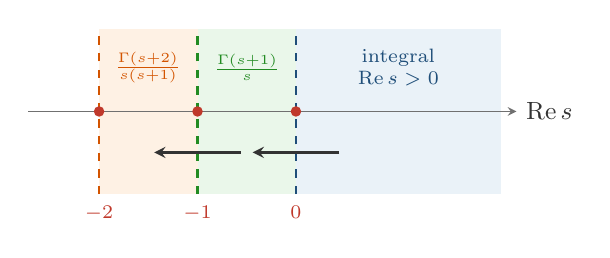
\begin{tikzpicture}[>=stealth,font=\small]
 \fill[lightblue] (0,-1.05) rectangle (2.6,1.05);
 \fill[lightgreen] (-1.25,-1.05) rectangle (0,1.05);
 \fill[lightorange!70] (-2.5,-1.05) rectangle (-1.25,1.05);
 \draw[darkgray!70,->] (-3.4,0) -- (2.8,0) node[right,text=darkgray] {$\Real s$};
 \draw[courseblue,dashed,thick] (0,-1.05) -- (0,1.05);
 \draw[ForestGreen,dashed,thick] (-1.25,-1.05) -- (-1.25,1.05);
 \draw[cayleyorange,dashed,thick] (-2.5,-1.05) -- (-2.5,1.05);
 % Poles at 0, -1, -2
 \foreach \x/\lab in {0/0, -1.25/-1, -2.5/-2} {
  \fill[cayleyred] (\x,0) circle (1.9pt);
  \node[below,font=\scriptsize,text=cayleyred] at (\x,-1.08) {$\lab$};
 }
 \node[font=\scriptsize,text=courseblue,align=center] at (1.3,0.56) {integral\\$\Real s>0$};
 \node[font=\scriptsize,text=ForestGreen,align=center] at (-0.62,0.56) {$\frac{\Gamma(s+1)}{s}$};
 \node[font=\scriptsize,text=cayleyorange,align=center] at (-1.88,0.56) {$\frac{\Gamma(s+2)}{s(s+1)}$};
 \draw[->,darkgray,thick] (0.55,-0.52) -- (-0.55,-0.52);
 \draw[->,darkgray,thick] (-0.70,-0.52) -- (-1.80,-0.52);
\end{tikzpicture}

\vspace{0.15em}
{\small Extending $\Gamma(s)$ strip by strip to the left via
$\Gamma(s)=\Gamma(s+n+1)/\bigl(s(s+1)\cdots(s+n)\bigr)$ introduces simple
poles at $s=0,-1,-2,\dots$.}
\end{minipage}
\end{lecturefigure}

More generally, for every integer $n\geq 0$, $\Gamma(s+n+1)$ is holomorphic
on the half-plane $\{\Real s > -(n+1)\}$, so setting
\begin{equation}\label{eq:gamma-ext-n}
 \Gamma(s) = \frac{\Gamma(s+n+1)}{s(s+1)\cdots(s+n)}
 \qquad (\Real s > -(n+1))
\end{equation}
defines a meromorphic function on $\{\Real s > -(n+1)\}$. By
\eqref{eq:gamma-iter}, the formula for $n+1$ agrees with the formula for
$n$ on $\{\Real s > -(n+1)\}$ (and both agree with the integral definition
on $\{\Real s > 0\}$). As $n$ ranges over all nonnegative integers, the
half-planes $\{\Real s > -(n+1)\}$ cover all of $\C$, producing a
meromorphic continuation of $\Gamma$ to $\C$ (unique by Section~1).

From \eqref{eq:gamma-ext-n}, the only possible poles in
$\{\Real s > -(n+1)\}$ are at $s=0,-1,\dots,-n$, each of order at most $1$.
At $s=-n$, the residue is
\[
 \operatorname{Res}_{s=-n}\Gamma(s)
 = \lim_{s\to -n} (s+n)\,\frac{\Gamma(s+n+1)}{s(s+1)\cdots(s+n)}
 = \frac{\Gamma(1)}{(-n)(-n+1)\cdots(-1)}
 = \frac{(-1)^n}{n!} \neq 0,
\]
confirming that every nonpositive integer $s=-n$ is indeed a simple pole.
Finally, the functional equation $s\,\Gamma(s)=\Gamma(s+1)$ holds for all
$s\in\C$ (outside poles) by uniqueness of analytic continuation.
\end{proof}

To conclude our study of $\Gamma(s)$ for now, we record one more classical
identity (which we take without proof) and deduce a crucial corollary that
we will need when we continue $\zeta(s)$ in Lecture~33.

\begin{lemma}[Euler's reflection formula]\label{lem:reflection}
For all $s\in\C\setminus\Z$,
\begin{equation}\label{eq:reflection}
 \boxed{\displaystyle
  \Gamma(s)\,\Gamma(1-s) = \frac{\pi}{\sin(\pi s)},}
\end{equation}
where $\sin(\pi s) = \dfrac{e^{i\pi s}-e^{-i\pi s}}{2i}$ for $s\in\C$.
\end{lemma}

\begin{corollary}[Zeros of $1/\Gamma(s)$]\label{cor:inv-gamma}
The function $1/\Gamma(s)$ extends to an \emph{entire} function on $\C$
whose only zeros are simple zeros at $s=0,-1,-2,-3,\dots$. In particular,
$\Gamma(s)$ has no zeros anywhere in $\C$.
\end{corollary}

\begin{proof}
Rearranging Euler's reflection formula \eqref{eq:reflection} gives
\[
 \frac{1}{\Gamma(s)} = \Gamma(1-s)\cdot\frac{\sin(\pi s)}{\pi}.
\]
Examine the two factors on the right-hand side:
\begin{itemize}
 \item By Theorem~\ref{thm:gamma-cont}, $\Gamma(1-s)$ is meromorphic on
       $\C$, with simple poles precisely where $1-s\in\{0,-1,-2,\dots\}$,
       i.e., at the positive integers $s=1,2,3,\dots$.
 \item The function $\frac{\sin(\pi s)}{\pi}$ is entire, with simple zeros
       precisely at all integers $s=0,\pm 1,\pm 2,\dots$ (since its
       derivative at $s=m\in\Z$ is $\cos(\pi m)=(-1)^m\neq 0$).
\end{itemize}
At each positive integer $s=1,2,3,\dots$, the simple pole of $\Gamma(1-s)$
cancels the simple zero of $\sin(\pi s)$, so the product has a removable
singularity there with nonzero value (namely $1/\Gamma(n)=1/(n-1)!$). Hence
$1/\Gamma(s)$ has \emph{no poles} anywhere in $\C$, and is therefore entire.

Moreover, $\Gamma(1-s)$ cannot vanish at any $s\notin\Z$ (otherwise
$\Gamma(s)\Gamma(1-s)=0$, contradicting $\pi/\sin(\pi s)\neq 0$), and at
each nonpositive integer $s=-n$ ($n\geq 0$) we have
$\Gamma(1-s)=\Gamma(n+1)=n!\neq 0$. Thus the zeros of $1/\Gamma(s)$ are
precisely the remaining simple zeros of $\sin(\pi s)$, namely
$s=0,-1,-2,-3,\dots$.
\end{proof}

\end{document}
